\section{Matched-Budget Component Attribution}
\label{sec:method}

\subsection{Setup and Notation}
\label{sec:setup}

Consider a rule-based trading system applied bar by bar to instrument $i$ at bar $t$. We decompose it into five
decision functions,
\begin{equation}
\mathcal{S} = (g, e, f, s, x),
\end{equation}
where the regime gate $g$ decides whether a bar is admissible, the entry rule $e \in \{-1, 0, +1\}$ fires a signal,
the filter $f$ decides whether a fired signal is taken, the sizing rule $s$ sets the position size, and the exit rule
$x$ closes an open position. In a purely rule-based control, $g$ admits every bar (or applies a rule such as an ADX
threshold), $f$ takes every signal, and $s$ sizes every trade at one unit. A \emph{component} $c$ replaces exactly one
of the five functions with a learned counterpart $\hat h_c$, giving the variant $\mathcal{S}_c$. The learned
counterpart is trained under a budget
\begin{equation}
B = (\mathcal{D}, \mathbf{x}, \mathcal{H}, \lambda, \tau),
\end{equation}
that is, training data $\mathcal{D}$, a feature map $\mathbf{x}_{i,t}$, a model class $\mathcal{H}$ with
hyperparameters $\lambda$, and a freeze date $\tau$ after which the model is never refit. The quantity MBCA
estimates for component $c$ on an out-of-sample window $W$ after $\tau$ is
\begin{equation}
\Delta\mathrm{SR}_c = \mathrm{SR}(\mathcal{S}_c; W) - \mathrm{SR}(\mathcal{S}; W),
\end{equation}
where $\mathrm{SR}$ is the annualized Sharpe ratio of the system's daily portfolio returns.

\subsection{The Matched Budget}

MBCA holds five elements fixed across every tested insertion point: the \emph{data} each model is trained and
evaluated on; the \emph{feature set} available to every learned component; the \emph{model class and
hyperparameters}, with no per-component tuning; the \emph{training and freeze discipline}, under which each model is
fit once and never refit on evaluation data; and the \emph{evaluation protocol and statistical test} used to call a
result significant. Only the insertion point varies between configurations (Table~\ref{tab:insertion}), so a
performance difference can be attributed to it rather than to feature engineering, tuning effort, or evaluation
leniency. The shared budget used in both studies is listed in Table~\ref{tab:budget}. A negative result under MBCA is
therefore a statement about this budget at this insertion point, not a claim that no learned model could help there.

\begin{table*}[!t]
\centering
\caption{The Insertion Points Tested, Their Rule-Based Controls, and Their Matched-Budget Learned Replacements}
\label{tab:insertion}
\footnotesize
\begin{tabular}{l p{4.3cm} p{6.3cm} l}
\toprule
Insertion point & Rule-based control & Learned replacement & Type \\
\midrule
Regime filter & ADX $\geq$ 25 gate (comparator), or no gate & classifier of trending vs.\ choppy bars gates entries & independent \\
Meta-labeling & take every fired signal & take a fired trade iff $\hat p^{\text{meta}} \geq 0.5$ & narrowing \\
Position sizing & one unit per trade & size each trade by $2\hat p^{\text{meta}} \in [0, 2]$ & narrowing \\
Entry & rule signal (JMA, SMA, Donchian, TSMOM, RSI(2)) & long and short target-before-stop classifiers & replacing \\
Exit & ATR stop and target, or trailing stop & continuation classifier plus a 3\,ATR safety stop & replacing \\
Meta-label + sizing & --- & meta-labeling filters, sizing re-weights the survivors & combination \\
\bottomrule
\end{tabular}
\end{table*}

\begin{table}[!t]
\centering
\caption{The matched budget shared by every learned component (read from the code).}
\label{tab:budget}
\footnotesize
\begin{tabular}{l p{5.2cm}}
\toprule
Item & Setting \\
\midrule
Features & ADX, ATR-normalized momentum, historical volatility, return $z$-score, backward-looking $R^2$, RSI, MACD histogram, KAMA slope (8, backward-only) \\
Model & LightGBM gradient-boosted trees on standardized features \\
n\_estimators & 200 \\
num\_leaves & 31 \\
max\_depth & 6 \\
learning\_rate & 0.05 \\
min\_child\_samples & 30 \\
class\_weight & balanced \\
random\_state & 42 \\
Small model (ablation) & n\_estimators = 50, num\_leaves = 7, max\_depth = 3 \\
\bottomrule
\end{tabular}
\end{table}


\subsection{A Taxonomy of Insertion Points}
\label{sec:taxonomy}

We classify each component by how much it can alter the set of trades the rule-based system would otherwise produce.
An \emph{independent} component gates admissibility orthogonally to the entry signal and can only reject bars; the ML
regime filter is independent, and a rule-based ADX gate serves as its comparator. A \emph{narrowing} component filters
or re-weights decisions the rule has already made and cannot create trades; meta-labeling and position sizing are
narrowing. A \emph{replacing} component substitutes the rule's own mechanism and can produce a materially different
trade set; learned entry and learned exit are replacing. The taxonomy implies an ex-ante hypothesis: because a
narrowing component can at worst remove the rule's good trades, it bounds its own downside and should produce smaller,
lower-variance effects than a replacing component, whose effects can be large in either direction.

\begin{figure*}[!t]
\centering
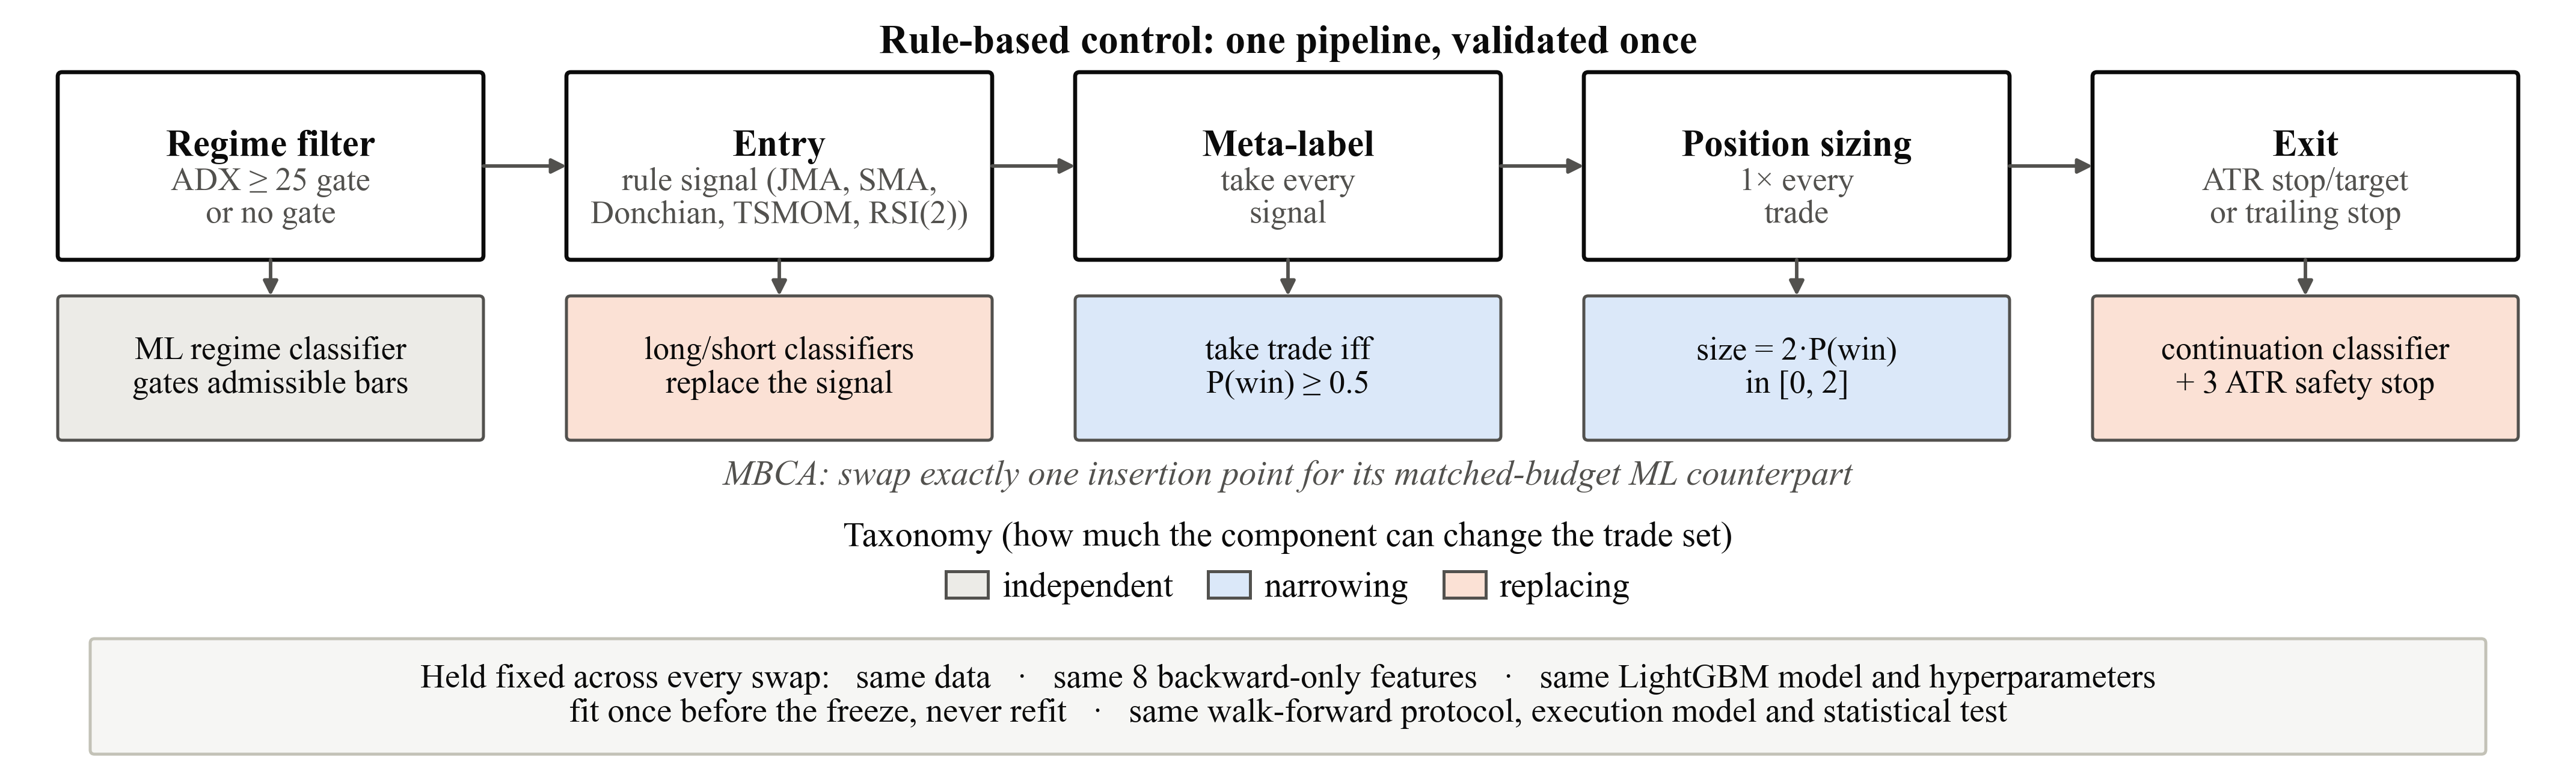
\includegraphics[width=7.14in]{figures/m_pipeline.png}
\caption{The MBCA experiment. Each of the five decisions of one rule-based pipeline (top) is swapped, one at a time,
for a learned counterpart (bottom, shaded by taxonomy), while the budget listed in the bottom band is held fixed
across every swap.}
\label{fig:pipeline}
\end{figure*}

\subsection{Components}
\label{sec:components}

Let $\mathbf{x}_{i,t} \in \mathbb{R}^{8}$ be the shared, backward-looking feature vector of instrument $i$ at bar
$t$ (Table~\ref{tab:budget}). Every classifier is a gradient-boosted tree ensemble \cite{ke2017lightgbm} with the same
hyperparameters, fit on standardized features.
\begin{itemize}
  \item \emph{ML regime filter:} entries are allowed iff
        $P(\text{trend}_{i,t} = 1 \mid \mathbf{x}_{i,t}) \geq 0.5$, where the label is one when the next 15 closes
        fit a straight line with $R^2 \geq 0.5$ (linearity). Study~1 also tests two alternative label definitions
        (excursion and move size); Study~2 pre-registers the linearity label only, so it cannot be chosen after the
        fact.
  \item \emph{ML meta-labeling:} at bars where the rule-based entry fires, the label is whether the trade the
        control would open is profitable; the trade is taken iff $\hat p^{\text{meta}}_{i,t} \geq 0.5$
        \cite{lopezdeprado2018afml}.
  \item \emph{ML position sizing:} the same frozen meta-label model, consumed continuously; every trade is sized
        $m_{i,t} = 2\hat p^{\text{meta}}_{i,t} \in [0, 2]$, so $\hat p = 0.5$ maps to one unit. No trade is added
        or removed.
  \item \emph{ML entry:} two classifiers estimate whether a long (short) bracket entered at $t$ with a 1.5\,ATR stop
        and a 3\,ATR target reaches the target first within 40 bars; the signal is the direction whose probability is
        larger and at least 0.5. This replaces the control's entry rule.
  \item \emph{ML exit:} two classifiers estimate whether an open long (short) position is still favourable ten bars
        ahead; the position exits at the first bar at which that probability falls below 0.5, or at a 3\,ATR safety
        stop. This replaces the control's exit rule.
  \item \emph{Meta-label + sizing:} meta-labeling filters and sizing re-weights the surviving trades. In Study~1 this
        pairing was identified after the fact as the most promising; in Study~2 it was pre-registered, so its Study~2
        result is an out-of-sample test of that choice.
\end{itemize}

\subsection{Protocol: Walk-Forward Selection and Freezing}
\label{sec:protocol}

Each classifier is fit exactly once, on data before its freeze date; training rows whose label window crosses the
freeze are excluded, and after the freeze the model only predicts. The parameters of the rule-based part of every
pipeline (signal lengths and stop multiples) are re-selected by the same anchored walk-forward procedure for the
control and for every variant: each instrument's history is split into five equal chronological folds, and the
parameter set with the best mean in-sample trade return, subject to a minimum trade count, is chosen on fold $k$ and
traded on fold $k+1$. Fig.~\ref{fig:timeline} shows the resulting training and out-of-sample windows of both studies.

\begin{figure}[!t]
\centering
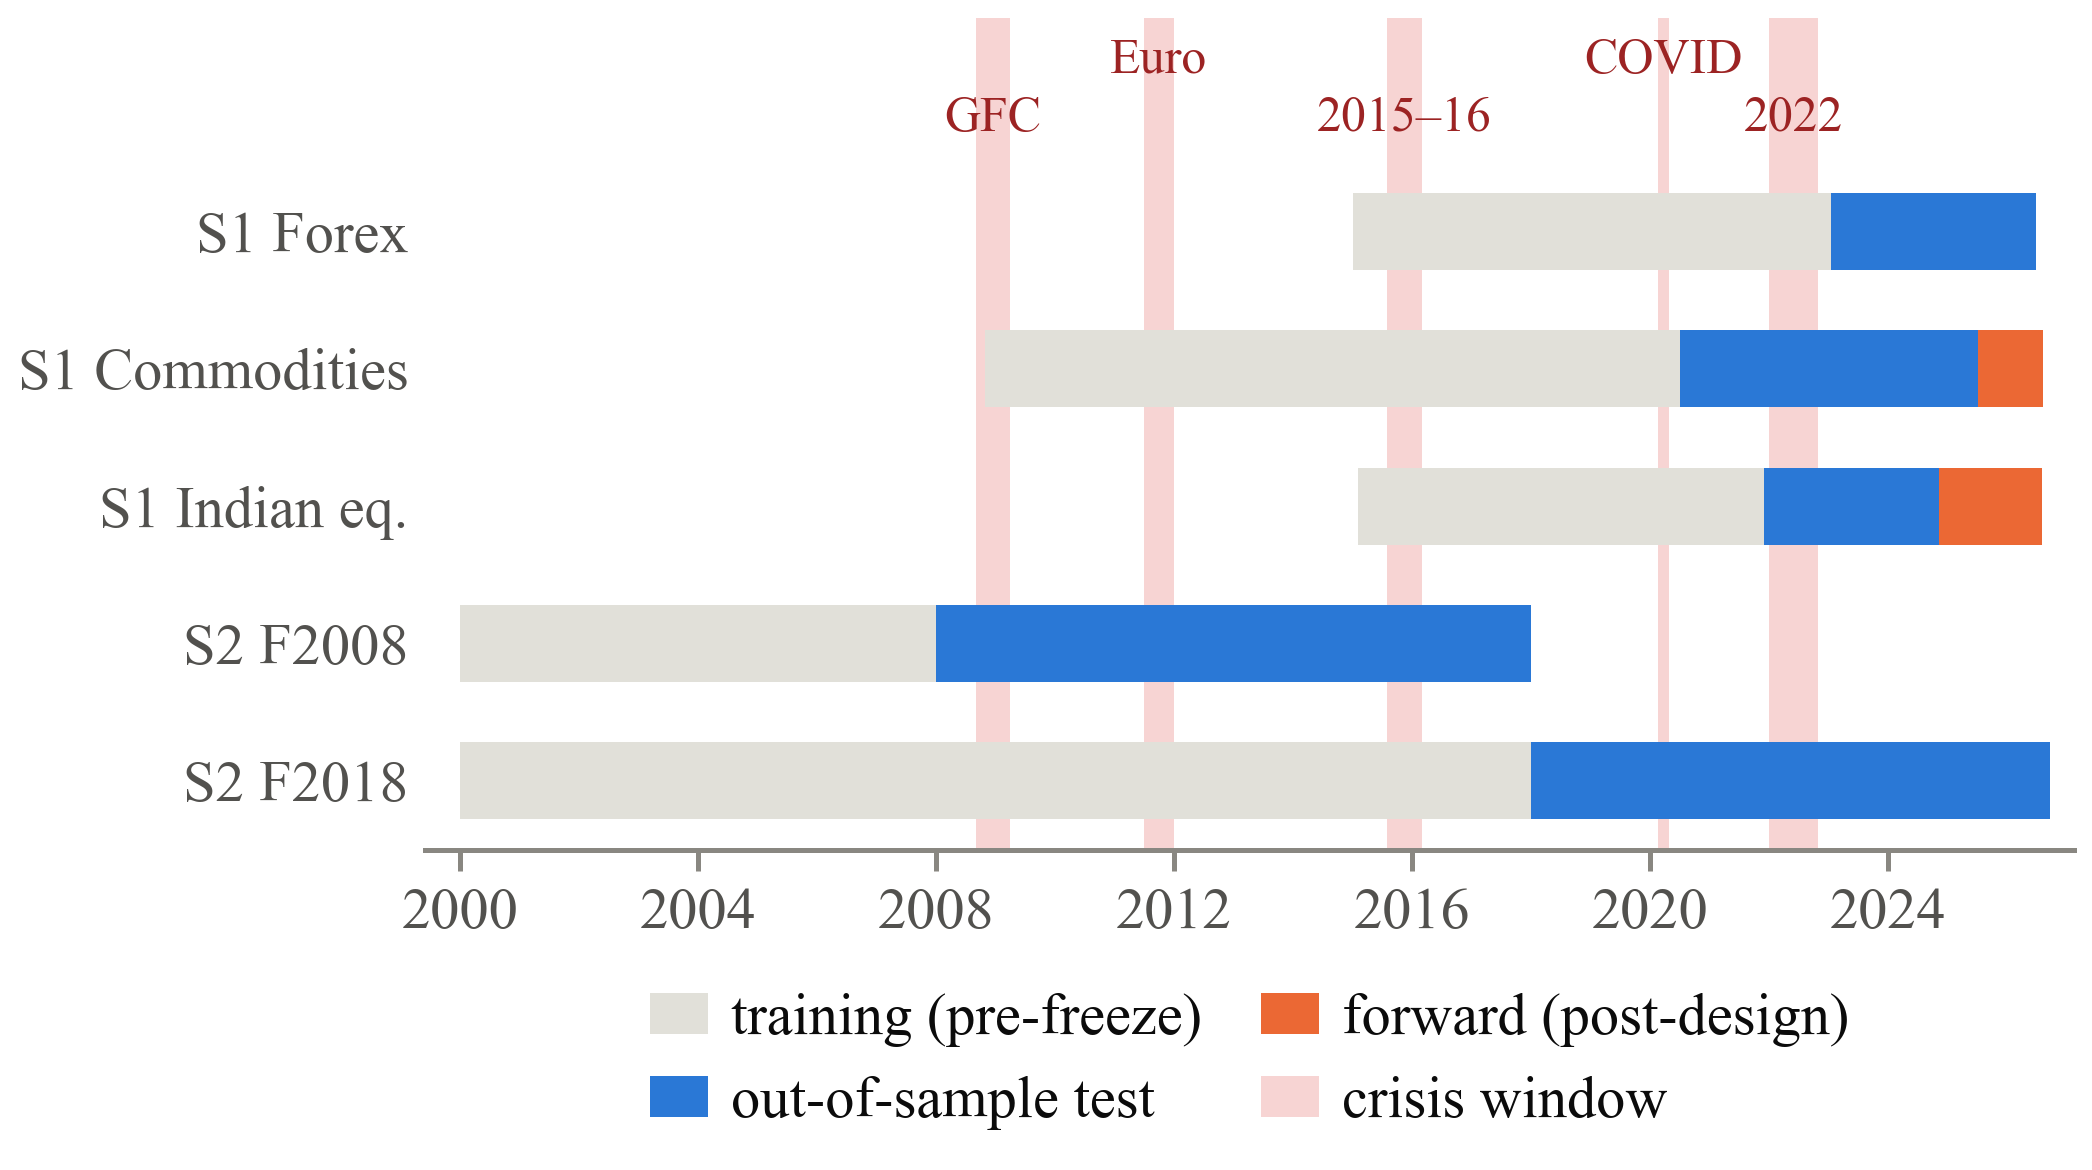
\includegraphics[width=3.487in]{figures/m_timeline.png}
\caption{Training and out-of-sample windows. Study~1 (S1) freezes each market at 70\% of its calendar span and adds a
forward window of data collected after the study was designed; Study~2 (S2) uses two independent freezes, F2008 and
F2018. Shaded bands mark the five pre-registered crisis windows.}
\label{fig:timeline}
\end{figure}
